\section{The Learning Algorithm}
\label{sec:learner:algorithm}

% Divide the section into two subsections: (i) filtering step, where steps 1 and 2 are included, and (ii) similarity-based outlier detection. In the second one, discuss different similarity metrics (edit distance, Jaccard similiarity, Tanimoto's similarity and reason why Jaccard is the best for us.

%Explain why pattern similarity and associated frequencies are the best candidates to learn EAMs. 

%Explain the approach to identify spurious action sequences (due to sensor noise and clustering errors).

%Explain the problems arose from using frequency as criterion.

%Conclude with the fact that only similarity of action sequences can be used in order to keep all variations performed by a user.

Summing up the conclusions obtained in Sections \ref{sec:learner:objectives} and \ref{sec:learner:relevant}, the task of learning EAMs can be seen as purging spurious action clusters from all the clusters extracted by the clustering process. The information that the $AML$ can use for this task is the action clusters themselves and associated occurrence frequencies. So the main idea is that action clusters contain all the action sequences performed by a user for each activity, but some of those clusters are spurious, due to sensor noise, user erratic behaviour and/or clustering errors. The $AML$ has to detect those spurious action sequences or outliers and remove them in order to keep only those action sequences that really represent an activity.

The designed learning algorithm works on the similarity between action sequences and their occurrence frequencies. A two-step process has been designed and implemented for that purpose: (i) the filtering step (Section \ref{subsec:learner:filtering}), where action sequences will be treated in terms of repeated actions and varied order of actions, and (ii) the similarity-based outlier detection step (Section \ref{subsec:learner:outlier}), where outlier action sequences will be detected in the similarity space and fused with the most similar action sequence taking their occurrence frequencies into account. The complete $AML$ algorithm and its final output are described in Section \ref{subsec:learner:complete}.

\subsection{Filtering step}
\label{subsec:learner:filtering}

If action clusters which define activities are carefully analysed, it can be seen that there are some clusters that contain repeated actions. Additionally, some clusters contain the same actions but in different order. In the ontology-based activity modelling approach described in Section \ref{sec:approach:ontology}, the activity models in terms of action properties do not contain repeated actions and the order in which actions are executed is not important (notice that descriptive properties do reflect this information, but they are not used when recognising activities). In consequence, two filtering steps are performed:

\begin{enumerate}
 \item Remove repeated actions into a sequence: some action sequences contain repeated actions. For instance, consider the sequence $S=\{a, b, a, c\}$. As repeated actions do not add any new information for activity modelling, they are removed. $S$ becomes $S' = \{a, b, c\}$. Notice that this step does not remove any action sequence of an activity. This step can be omitted depending on how activity models are used by the activity recognition system. The work presented in this paper is based on the knowledge-driven approach developed by Chen et al. in \cite{Chen2012a}. This activity recognition system does not consider repeated actions in the recognition phase, so activity models do not have this information. However, if the recognition system is sensitive to repeated actions, the learning algorithm can be easily modified to omit this first filtering step.
 
 \item Fuse equal action sequences: some action sequences contain the same actions, but in different order. For example, $S_1 = \{a, b, c \}$ and $S_2 = \{b, c, a\}$. The order of actions is not important for activity models, so both sequences are fused. Two action sequences are equal if:
 
 \begin{equation}
 \label{eq-equal}
  S_1 \cap S_2 = S_1 \cup S_2
 \end{equation}

 Any two action sequences that fulfil equation \ref{eq-equal} are fused. Fusing implies removing one of the action sequences and to sum occurrence frequencies of both action sequences to assign it to the fused sequence. Thus from two sequences a resultant sequence will remain, reducing the number of valid action sequences.

\end{enumerate}

As a consequence of the filtering step, the number of clusters for an activity will be equal or less than the clusters provided as input.


\subsection{Similarity-based outlier detection step}
\label{subsec:learner:outlier}
The idea behind the similarity-based outlier detection is simple: all the action sequences describing the same activity will have their own similarity distribution depending on the varied ways of performing the activity by a concrete user. Spurious action sequences will be those which are very similar to valid action sequences, and their difference will be related to sensor noise or clustering errors. Hence, if outliers are detected in the similarity space between action sequences, those outliers will point to spurious action sequences. 

The first thing needed to apply the idea introduced above is a similarity measure for two action sequences. The literature offers a lot of similarity measures to compare two sequences. However, many of them take into account the order of the elements of both sequences, such as the Levenshtein distance \cite{Levenshtein1966}, Hamming distance \cite{Hamming1950} or most frequent $k$ characters \cite{Seker2014}. As explained in Section \ref{subsec:learner:filtering}, the order of actions is not relevant for ontology-based activity modelling, thus order-based similarity measures are not useful to detect outlier action sequences.

There are two similarity measures that do not care about the order of the elements of sequences, namely the Jaccard coefficient \cite{A.K.Jain1988} and the S{\o}rensen-Dice coefficient \cite{Sorensen1948}. The Jaccard coefficient measures similarity between finite sample sets, and is defined as the size of the intersection divided by the size of the union of the sample sets:

\begin{equation}
\label{eq-jaccard}
  Jaccard(A, B) = \frac{|A \cap B|}{|A \cup B|}
 \end{equation}

It can be seen that $Jaccard(A, B) \in [0, 1]$. Moreover, if sequences $A$ and $B$ are equal, $Jaccard(A, B) = 1$. If $A$ and $B$ are empty sequences the Jaccard coefficient is defined to be 1.

The S{\o}rensen-Dice coefficient is very similar to the Jaccard coefficient. It is denoted as $QS$ and defined as the size of the intersection multiplied by two divided by the sum of the elements of both sequences:

\begin{equation}
 QS(A, B) = \frac{2 |A \cap B|}{|A| + |B|}
\end{equation}

Similarly to Jaccard coefficient, $QS(A, B) \in [0, 1]$. Since it does not satisfy the triangle inequality, the S{\o}rensen-Dice coefficient can be considered a semimetric version of the Jaccard coefficient. This coefficient is mainly useful for ecological community data. Justification for its use is primarily empirical rather than theoretical, although it can be justified theoretically as the intersection of two fuzzy sets \cite{Roberts1986}. 

For the outlier detection step, the Jaccard coefficient has been selected, because it is a theoretically well founded measure which can be seen as the basis of the S{\o}rensen-Dice coefficient. So the similarity between two action sequences is given by the Jaccard coefficient of both sequences. The value 1 denotes that both sequences are equal, whereas 0 means that there is nothing in common between both sequences. Notice that due to the filtering step (Section \ref{subsec:learner:filtering}) there will not be equal action sequences at this stage, hence value 1 will not appear. Similarly, having a 0 value is also impossible, since all the action sequences describing the same activity share at least the actions contained in their IAMs. 

% TODO -> enhance the description of the outlier detection algorithm!
The similarity-based outlier detection is an iterative algorithm which uses the Jaccard coefficient to calculate the similarity between action sequences. The algorithm calculates the so called \textit{Jaccard Matrix} ($JM$), which is a square matrix of all action sequences that remain from the previous iteration (in the case of the first iteration, action sequences coming from the filtering step in Section \ref{subsec:learner:filtering}). $JM_{i, j}$ stores the Jaccard coefficient for action sequences $S_i$ and $S_j$. 

\begin{equation}
JM = \left(
\begin{array}{ccc}
 Jaccard(S_0, S_0) & \cdots & Jaccard(S_0,S_N) \\
 \vdots & \ddots & \vdots \\
 Jaccard(S_N,S_0) & \cdots & Jaccard(S_N,S_N) 
\end{array}
\right)
\end{equation}

The diagonal of $JM$ is 1, since two equal action sequences' Jaccard coefficient is 1 ($\forall i, j : i = j \rightarrow Jaccard(S_i, S_j) = 1$). Diagonal values do not provide any information for outlier detection, so they are removed. Removing diagonal values from $JM$, $\hat{JM}$ is obtained. The $\hat{JM}$ matrix has the information of the similarity of all action sequences detected for a concrete activity. Figure \ref{fig-similarity} shows a plot of the similarity values between 11 action sequences, taken from a real example (they are representing the activity MakePasta for a concrete user). The idea of the similarity-based outlier detection is to identify similarity values that stand out among everyone else; then, take the action sequences that are represented by those outlier similarity values and fuse them.  

\begin{figure}[htbp]
\centering
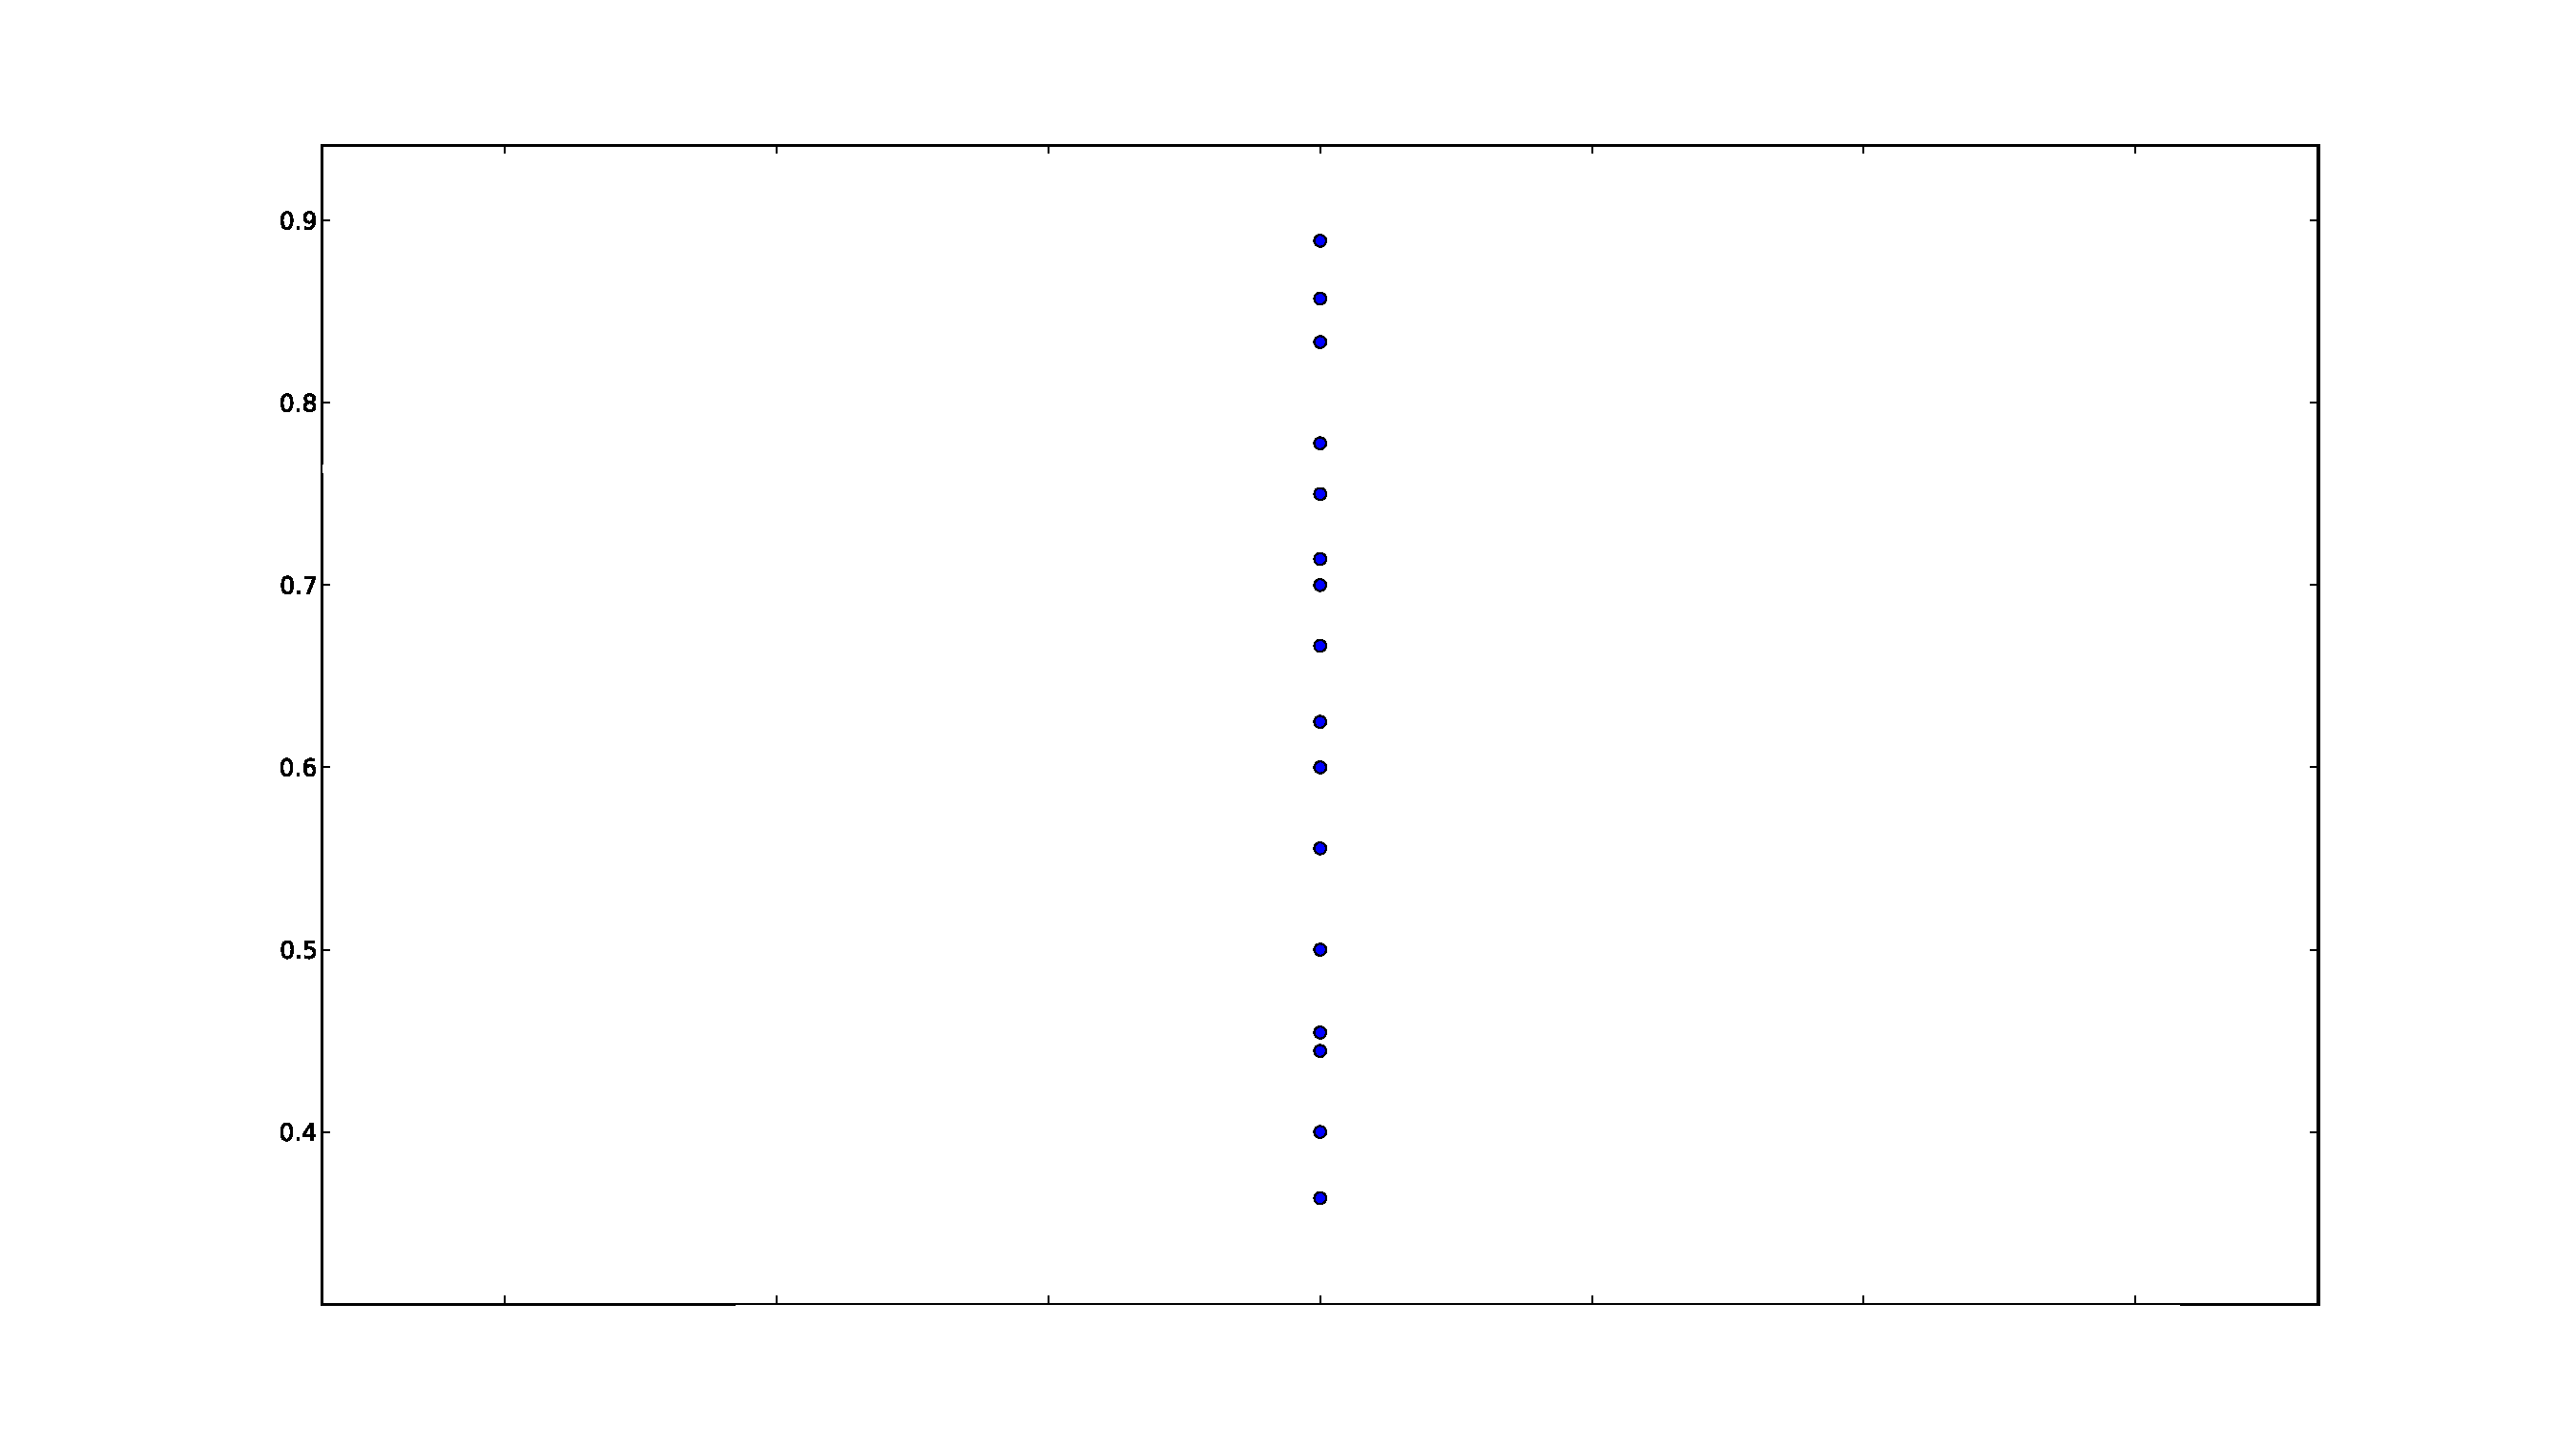
\includegraphics[width=\textwidth]{similarity_plot.pdf}
    \caption{Jaccard coefficient-based similarity values for 11 action sequences detected for a concrete activity and a concrete user.}
    \label{fig-similarity}
\end{figure}

To detect outlier similarity values, a statistical approach has been defined. Fixing a static threshold value for every activity is not appropriate, since some activities may contain many actions, whereas others are performed by means of few actions. So a difference of a single action in a ``short'' activity cannot have the same weight as in a ``long'' activity (short and long are here used to refer to the number of actions of activities). Furthermore, some users may execute very different action sequences to perform the same activity, while others may only add slight variations. In consequence, the outlier detection method has to calculate a threshold for every action sequence group describing an activity. 

The strategy followed to calculate the threshold is based on the median value of the $\hat{JM}$ matrix. The median is the numerical value separating the higher half of a data sample from the lower half. The median of a finite list of numbers can be found by arranging all the observations from lowest value to highest value and picking the middle one. If there is an even number of observations, then there is no single middle value; the median is then usually defined to be the mean of the two middle values. The median has been chosen rather than the mean, because the median is a robust estimator which is less influenced by outliers than the mean value. Using the median allows detecting the similarity ``centre of gravity'' minimising the influence of outliers. %Once the median of $\hat{JM}$ is calculated, the standard deviation of similarity values to the median is calculated. Summing the median and the standard deviation value an appropriate threshold for outlier detection is determined:

% The standard deviation is not being used really. We are using the average absolute deviation about median

Once the median of $\hat{JM}$ measures the central tendency, another statistic is needed to capture the dispersion of similarity in $\hat{JM}$. Two good candidates to measure the dispersion in univariate datasets have been found in the literature \cite{Hoaglin1983}. The first one is the median absolute deviation (MAD) and it is defined as the median of the absolute deviations from the data's median:

\begin{equation}
\label{eq-mad}
 MAD = median_i (|X_i - median_j(X)|)
\end{equation}

The MAD is a measure of statistical dispersion. Moreover, the MAD is a robust statistic, being more resilient to outliers in a dataset than the standard deviation. In the standard deviation, the distances from the mean are squared, so large deviations are weighted more heavily, and thus outliers can heavily influence it. In the MAD, the deviations of a small number of outliers are irrelevant.

There is another dispersion measure, which is known as the average absolute deviation about median (ADM). The ADM offers a direct measure of the scale of a random variable about its median and it is defines as:

\begin{equation}
 \label{eq-adm}
 ADM = E_i |X_i - median(X)|
\end{equation}

Both the MAD and the ADM can be used to establish a proper threshold and identify outlier similarity values. However, in the current implementation the ADM has been chosen. It is true that the ADM is more influenced by outliers than the MAD, but from the point of view of the conservative approach to learning, the ADM is more suitable. The reason is that the MAD can have a value of zero if there are some similarity values with the same values as the median. This fact makes that the median itself could be taken as the threshold, which is quite aggressive. On the other hand, the only way the ADM can be zero is to have all similarity values being equal to the median. Moreover, it can be shown mathematically that the MAD of a given dataset will always be less or equal to the ADM, so the MAD is more aggressive in all the cases. 

Due to those reasons, the ADM has been chosen to establish a statistical threshold to separate normal similarity values from outlier values. The threshold is defined as:

\begin{equation}
\label{eq-stat-threshold}
 \theta_S = median(\hat{JM}) + ADM(\hat{JM})
\end{equation}

As the threshold in equation \ref{eq-stat-threshold} has been calculated using statistical approaches, it is denoted as $\theta_S$. Applying equation \ref{eq-stat-threshold} to the similarity values plotted in the example of Figure \ref{fig-similarity}, a threshold can be calculated. This threshold is depicted in Figure \ref{fig-threshold-calc}. Similarity values above the threshold can be considered as outliers. 

\begin{figure}[htbp]
\centering
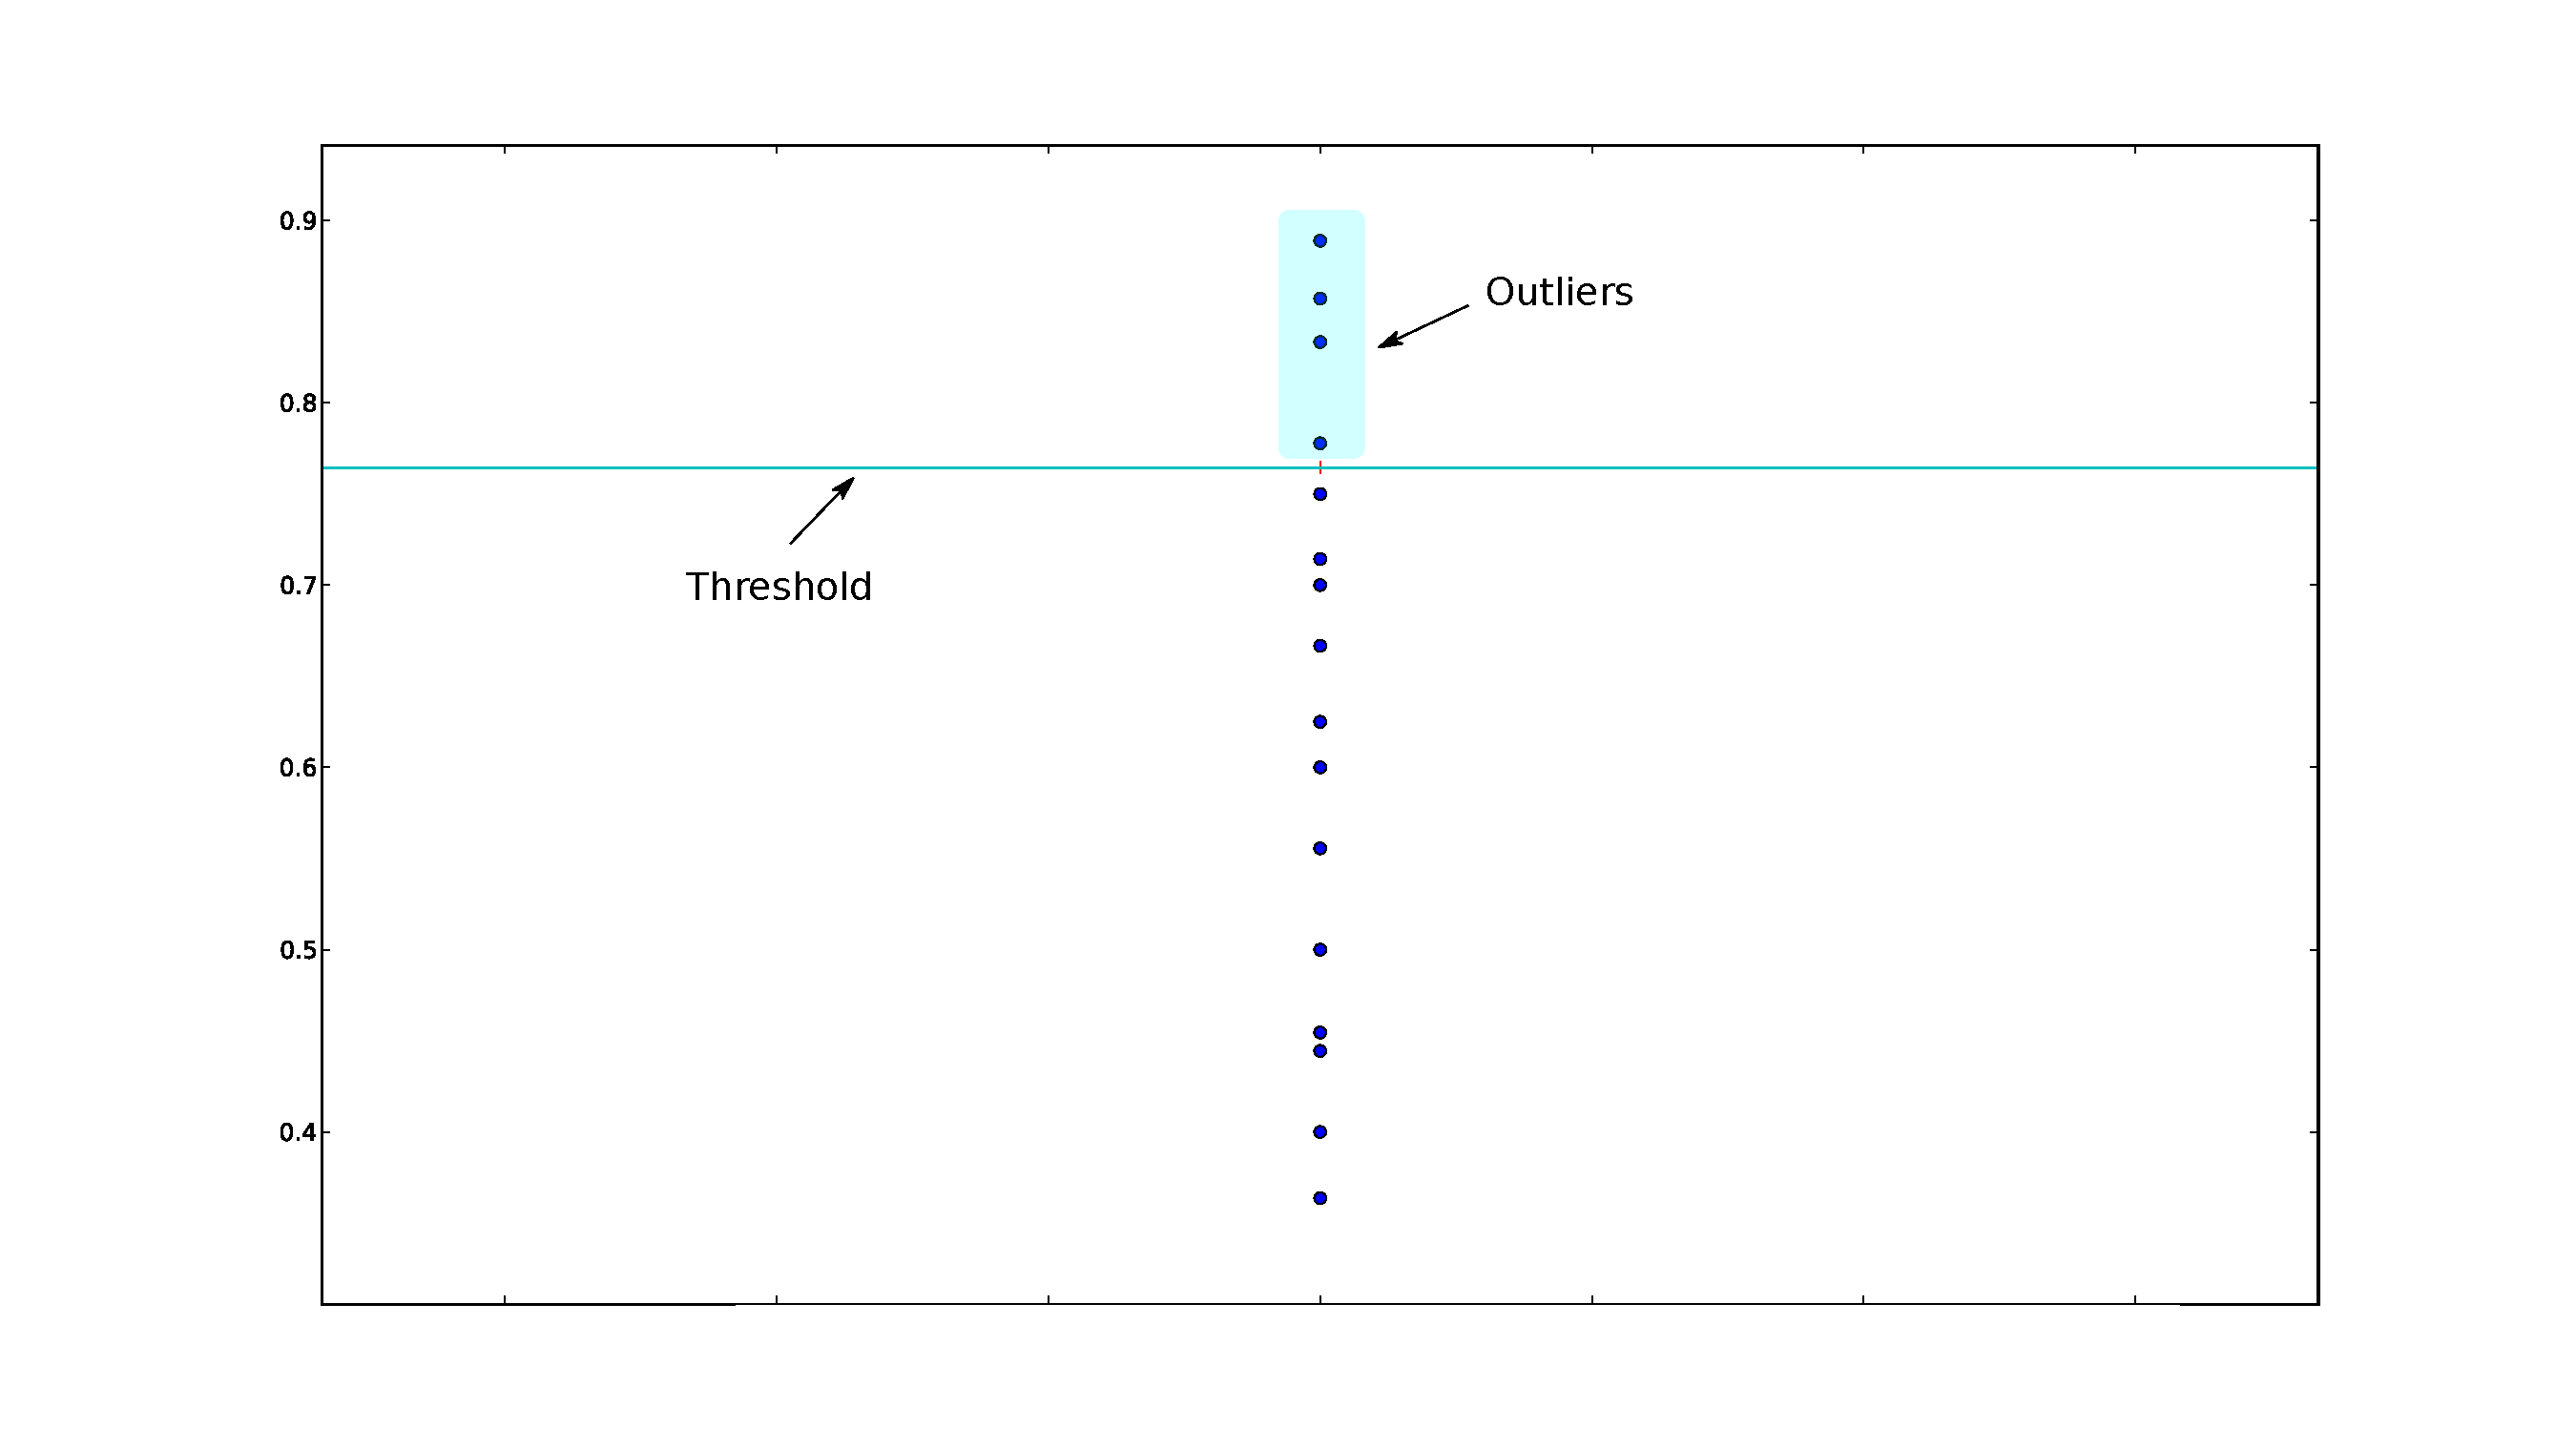
\includegraphics[width=\textwidth]{threshold_calculation.pdf}
    \caption{The threshold calculated for the similarity values of 11 action sequences representing a concrete activity.}
    \label{fig-threshold-calc}
\end{figure}

Statistical approaches work well when ``a lot of'' data is available. But when ``few'' data is available, statistic-based approaches may extract weak conclusions. For example, imagine the following action sequences are being analysed by $AML$ for the activity MakePasta (this example is extracted from a real experiment):

\begin{equation*}
 \begin{split}
  S_1 = \{ turnOnTap, useCookingAppliance, hasPasta,\\ useCookingUtensil, hasPesto \} \\
  S_2 = \{ hasPasta, useCookingAppliance, turnOnTap,\\ hasBacon, hasCream, useCookingUtensil \} \\
  S_3 = \{ turnOnTap, useCookingAppliance, hasPasta,\\ useCookingUtensil, hasTomato \}
 \end{split}
\end{equation*}

The difference between $S_1$ and $S_3$ is that the user adds pesto in the first and tomato in the second, i.e. only one action out of five. All three action sequences are really performed by the user and they should not be removed or fused. However, if $\theta_S$ is calculated for the group of action sequences, a value of 0.6 is obtained. Considering that $Jaccard(S_1, S_3) = 0.66$, action sequences $S_1$ and $S_3$ should be fused, thus removing one of the action sequences which has actually been performed by the user. Notice that detecting outliers using statistical approaches on three samples is not generally feasible. Removing one of the action sequences would contradict the conservative policy selected for the $AML$, where the priority is given to learning all real action sequences performed by a user. Hence, a defensive mechanism for those cases is adopted. The threshold to identify outliers is defined as:

\begin{equation}
\label{eq-threshold}
 \theta = max \{ \theta_S, \lambda \}
\end{equation}

\noindent where $\lambda$ is a fixed value. The idea of this approach is to state a similarity value that acts as a minimum value for action sequences to be fused. In the experiments performed in this dissertation $\lambda = 0.75$ (Chapter \ref{cha:evaluation}). If $\lambda$ is set to higher values, the $AML$ will be even more conservative, whereas decreasing $\lambda$ will make the $AML$ rely more on the statistic-based approach ($\theta_S$). Figure \ref{fig-both-thresholds} shows both thresholds, $\theta_S$ and $\lambda$, for the example of MakePasta activity and its three action sequences. Notice that $Jaccard(S_1, S_2) = Jaccard(S_2, S_3)$ and thus, only one point is depicted in the graphic. It can be seen clearly how using only $\theta_S$, $Jaccard(S_1, S_3)$ is an outlier and in consequence, sequences $S_1$ and $S_3$ would be incorrectly fused. But using equation \ref{eq-threshold} and taking the maximum of both thresholds, there is not any outlier and hence all three sequences are kept as valid activity models. 

\begin{figure}[htbp]
\centering
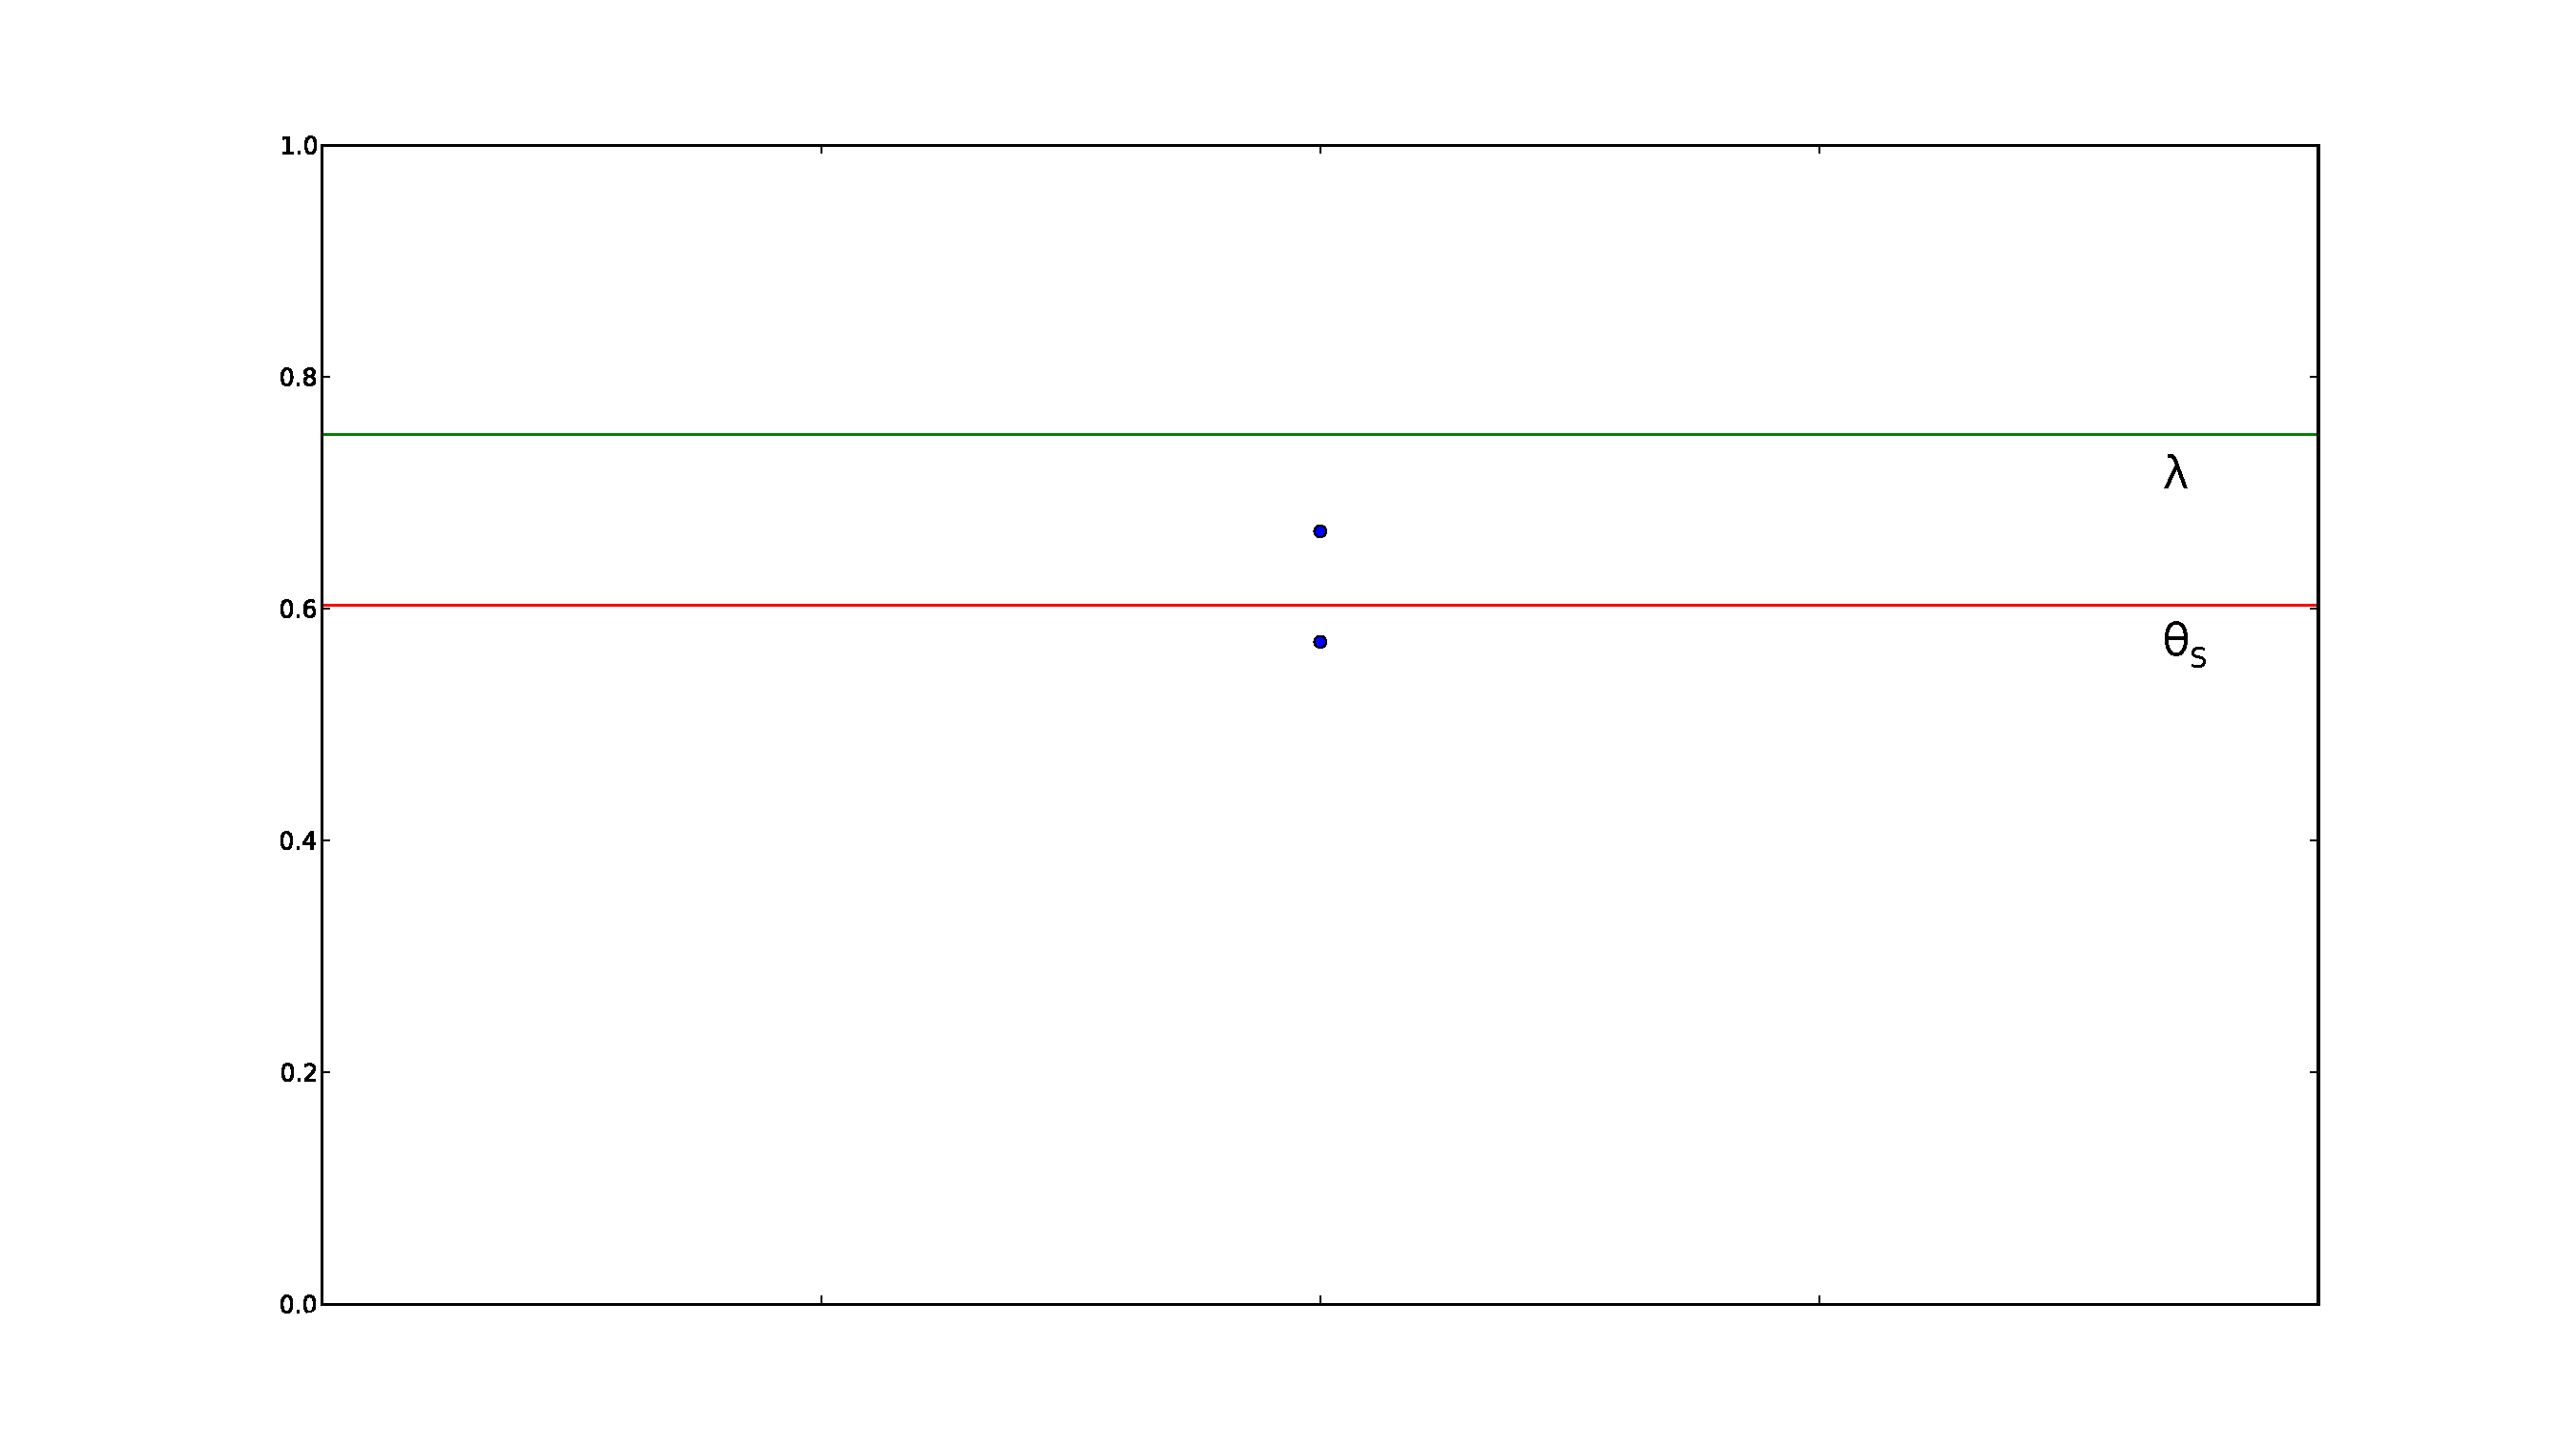
\includegraphics[width=\textwidth]{both_thresholds.pdf}
    \caption{Both thresholds depicted in an example of few available data: $\theta_S$ and $\lambda$.}
    \label{fig-both-thresholds}
\end{figure}

The similarity-based outlier detection algorithm is an iterative process that fuses sequences whose Jaccard coefficient is higher than $\theta$, until no sequences can be fused. Fusing implies defining a function which returns a single action sequence having as input two different action sequences. In the case of the $AML$ a fusing heuristic has been adopted, which states that given two action sequences to be fused, the lower frequency sequence is a spurious variation of the higher frequency sequence. In consequence, the higher frequency action sequence is the valid one and the function will return it as the fused action sequence. 

\begin{equation}
\label{eq-fusion}
 Fusion(S_i, S_j) = \left\{
\begin{array}{cc}
 S_i, & \mbox{if } f_{S_i} \geq f_{S_j} \\
 S_j, & \mbox{otherwise}
\end{array}
\right.
\end{equation}

\noindent where $f_{S_i}$ is the occurrence frequency of action sequence $S_i$. The fused action sequence will have a new occurrence frequency which is calculated as the sum of the occurrence frequencies of fused sequences: $f_{S_{fused}} = f_{S_i} + f_{S_j}$. 

\subsection{The complete AML algorithm}
\label{subsec:learner:complete}

Combining the filtering step described in Section \ref{subsec:learner:filtering} and the similarity-based outlier detection step described in Section \ref{subsec:learner:outlier}, the complete $AML$ algorithm can be built. Its inputs are the activity clusters file, where the result of the clustering process is given, and the fixed threshold $\lambda$. Algorithm \ref{alg:aml} shows the $AML$ algorithm written in pseudo-code.  

\begin{algorithm}
 \caption{$AML$ algorithm for learning extended activity models}
 \label{alg:aml}
 \begin{algorithmic}
 \REQUIRE activity\_clusters, $\lambda$
 \ENSURE learned\_action\_sequences
 \STATE $activities \leftarrow obtainActivities(activity\_clusters)$
 \FORALL{$activity \in activities$}
   \STATE $action\_sequences \leftarrow obtainSequences(activity, activity\_clusters)$
   \STATE // The filtering step
   \STATE $action\_sequences \leftarrow filteringStep(action\_sequences)$
   \STATE // The similarity-based outlier detection step
   \REPEAT
     \STATE $JM \leftarrow jaccardMatrix(action\_sequences)$
     \STATE $\hat{JM} \leftarrow removeDiagonal(JM)$
     \STATE $\theta_S \leftarrow calculateStatisticThreshold(\hat{JM})$
     \STATE $outliers \leftarrow detectOutliers(\hat{JM}, \theta_S, \lambda)$
     \STATE $action\_sequences \leftarrow fuseSequences(action\_sequences, outliers)$
   \UNTIL{$outliers = \emptyset$}
   \STATE $learned\_action\_sequences \leftarrow addActivityModel(activity, action\_sequences)$
 \ENDFOR
 \RETURN $learned\_action\_sequences$ 
 \end{algorithmic}
\end{algorithm}

The output of the $AML$ algorithm is the so called learned action sequences file, stored in a JSON file in the current implementation. This file contains the extended activity models for every activity defined in the context model. An example can be seen in Figure \ref{fig-aml-output}, where two complete and specialised models for activity MakePasta are provided. The example is extracted from a real experiment, where the user prepares pasta \textit{carbonara} more or less the 50\% of times and pasta with tomato sauce also around 50\% of times. Looking at the action sequences, the different ways of preparing pasta can be distinguished. In the first way, labelled by the user as pasta \textit{carbonara}, bacon and cream are used by the user (actions \textit{hasBacon} and \textit{hasCream}). In the second way, action \textit{hasTomato} appears, which makes reference to the usage of tomato sauce. Notice also that the first action sequence contains an \textit{openFridge} action, which suggests that some of the ingredients are stored in the fridge. This does not happen in the second action sequence, where all the ingredients are taken from the food store (action \textit{openStore}).

\begin{figure}[htbp]
\begin{small}
\begin{lstlisting}
 "MakePasta": {
     "1": [          
             0.5074626865671642, 
             [
                  "hasPasta", 
                  "useCookingAppliance", 
                  "hasBacon", 
                  "turnOnTap", 
                  "openFridge", 
                  "openStore", 
                  "hasCream", 
                  "useCookingUtensil"
              ]
            ],
     "2": [
             0.49253731343283574, 
             [
                  "hasTomato", 
                  "hasPasta", 
                  "useCookingAppliance", 
                  "turnOnTap", 
                  "openStore", 
                  "useCookingUtensil"
             ]
            ]        
    }, 

\end{lstlisting}
\end{small}
\caption{Example of the output of the $AML$ algorithm. Two specialised and complete models for MakePasta activity are depicted. As their semantic tags are not known, they are tagged with numbers 1 and 2.}
\label{fig-aml-output}
\end{figure}


